\documentclass{article}
\usepackage[margin=1in]{geometry}
\usepackage{tikz}
\begin{document}
\def\eps{0.15}
\def\rad{3pt}
\def\xtick#1{\draw[thick] (#1,0) +(0,\eps) -- +(0,-\eps) node[below] {#1};}
\def\ytick#1{\draw[thick] (0,#1) +(\eps,0) -- +(-\eps,0) node[left]  {#1};}
  
\begin{center}
  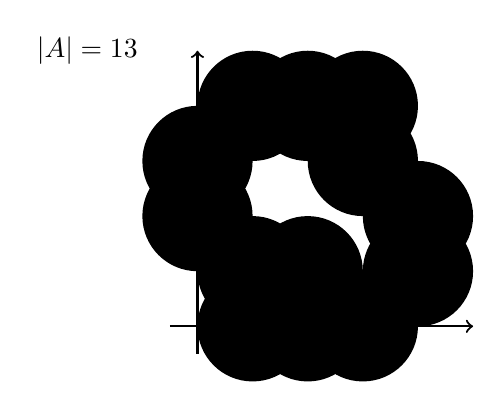
\begin{tikzpicture}[scale=0.7]
    \draw[thick,->] (-0.5,0) -- (5,0); 
    \draw[thick,->] (0,-0.5) -- (0,5);
    \foreach \x in {1,...,4} {
      \xtick\x
      \ytick\x
    }
    
    \foreach \x/\y in {0/2, 0/3, 1/0, 1/1, 1/4, 2/0, 2/1, 2/4, 3/0, 3/3, 3/4, 4/1, 4/2}
    {
      \fill (\x,\y) circle (\rad);
    }
    \node at (-2,5) {$|A| = 13$};
  \end{tikzpicture}
\end{center}

\begin{center}
  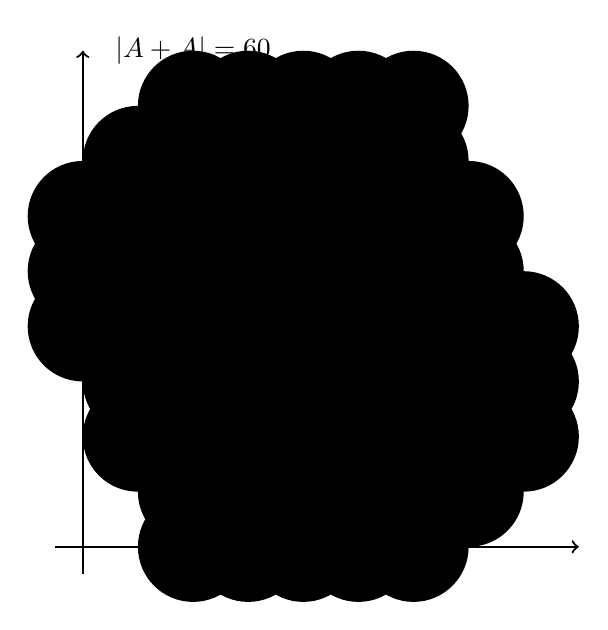
\begin{tikzpicture}[scale=0.7]
    \draw[thick,->] (-0.5,0) -- (9,0); 
    \draw[thick,->] (0,-0.5) -- (0,9);
    \foreach \x in {1,...,8} {
      \xtick\x
      \ytick\x
    }
    \node at (2,9) {$|A+A| = 60$};

    \foreach \x/\y in 
    {0/4, 0/5, 0/6, 1/2, 1/3, 1/4, 1/6, 1/7, 2/0, 2/1, 2/2, 2/3, 2/4, 2/5, 2/6, 2/7, 2/8, 
      3/0, 3/1, 3/2, 3/3, 3/4, 3/5, 3/6, 3/7, 3/8, 4/0, 4/1, 4/2, 4/3, 4/4, 4/5, 4/7, 4/8, 
      5/0, 5/1, 5/2, 5/3, 5/4, 5/5, 5/6, 5/7, 5/8, 6/0, 6/1, 6/2, 6/3, 6/4, 6/5, 6/6, 6/7, 6/8, 
      7/1, 7/2, 7/4, 7/5, 7/6, 8/2, 8/3, 8/4}
    {
      \fill (\x,\y) circle (\rad);  
    }    
  \end{tikzpicture}~~~~
  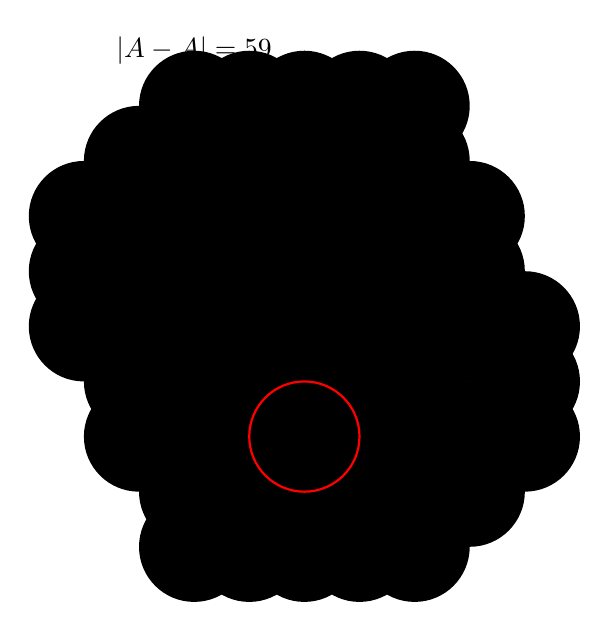
\begin{tikzpicture}[scale=0.7]
    \draw[thick,->] (-5,0) -- (5,0); 
    \draw[thick,->] (0,-5) -- (0,5);
    \foreach \x in {1,...,4} {
      \xtick\x
      \ytick\x
      \xtick{-\x}
      \ytick{-\x}
    }

    \node at (-2,5) {$|A-A| = 59$};

    \foreach \x/\y in 
    {0/0, 0/1, 0/-1, 0/3, 0/-3, 0/4, 0/-4, 1/0, -1/0, 1/1, 1/-1, -1/1, -1/-1,
      1/2, 1/-2, -1/2, -1/-2, 1/3, 1/-3, -1/3, -1/-3, 1/4, 1/-4, -1/4, -1/-4,
      2/0, -2/0, 2/1, 2/-1, -2/1, -2/-1, 2/2, 2/-2, -2/2, -2/-2, 2/3, 2/-3,
      -2/3, -2/-3, 2/4, 2/-4, -2/4, -2/-4, 3/0, -3/0, 3/1, -3/-1, 3/2, 3/-2,
      -3/2, -3/-2, 3/-3, -3/3, 4/0, -4/0, 4/-1, -4/1, 4/-2, -4/2}
    {
      \fill (\x,\y) circle (\rad);
    }

    \draw[thick,red] (0,-2) circle (\rad);
  \end{tikzpicture}
\end{center}

\end{document}
